\section{Results}

\subsection{Microsimulation Non-take-up}
Our microsimulation results indicate that the non-take-up-rate of BAföG, among theoretically eligible students ranged from approximately 50--70\% across the survey years 2007--2021, with an average of 60\%  (Table \ref{table:microsimulation-ntu}).

These estimates are broadly in line with previous findings on non-take-up of social benefits in Germany, which generally falls between 40--67\%, depending on the program and time period (see Table \ref{table:NTU-studies}). 
While our estimates are broadly consistent with prior research, they are noticeably higher than the 36--40\% non-take-up rate for BAföG reported by \cite{herber_non-take-up_2019}, who also use SOEP survey data, but for the period 2002--2013.

This discrepancy may be attributable to several factors, including differences in the estimation of theoretical eligibility. These factors include the specific SOEP variables used to capture income and reported BAföG receipt, the time periods under study (with our analysis covering 2007--2021, compared to \cite{herber_non-take-up_2019}, which covers 2002--2013), as well as other differences in the microsimulation design and modeling approach.



\begin{table}[htbp]
\centering
\begin{tabular}{l@{\hspace{2em}}r@{\hspace{2em}}r}
\toprule
\textbf{Year} & \textbf{Non-Take-Up}  &  \textbf{Beta Error}  \\
              & \(\Pr(\text{NTU} =1\,|\,\text{M} = 1)\) & \(\Pr(\text{TU} = 1\,|\,\text{M} = 0)\) \\
\midrule
2007 & 58.0 & 15.9 \\
2008 & 60.4 & 19.8 \\
2009 & 58.0 & 19.4 \\
2010 & 53.0 & 21.9 \\
2011 & 51.4 & 17.8 \\
2012 & 48.4 & 20.8 \\
2013 & 51.0 & 11.9 \\
2014 & 52.6 & 14.7 \\
2015 & 72.1 & 12.8 \\
2016 & 58.2 & 15.5 \\
2017 & 64.0 & 7.0 \\
2018 & 68.8 & 11.5 \\
2019 & 69.0 & 11.1 \\
2020 & 69.3 & 13.0 \\
2021 & 69.9 & 17.6 \\
\midrule
\textbf{Average} & \textbf{60.0} & \textbf{15.8} \\
\bottomrule
\end{tabular}
\caption{Non-Take-Up and Beta Error Rates by Survey Year (\%). Non-take-up is the share of theoretically eligible students (\(M=1\)) who do not receive BAföG; beta error is the share of theoretically ineligible students (\(M=0\)) who do receive BAföG.}
\caption*{\small{Notes: SOEP v39, 2007--2021, weighted with individual weights}}
\label{table:microsimulation-ntu}
\end{table}


\begin{figure}[htbp]
  \centering
  \begin{subfigure}[t]{0.48\linewidth}
    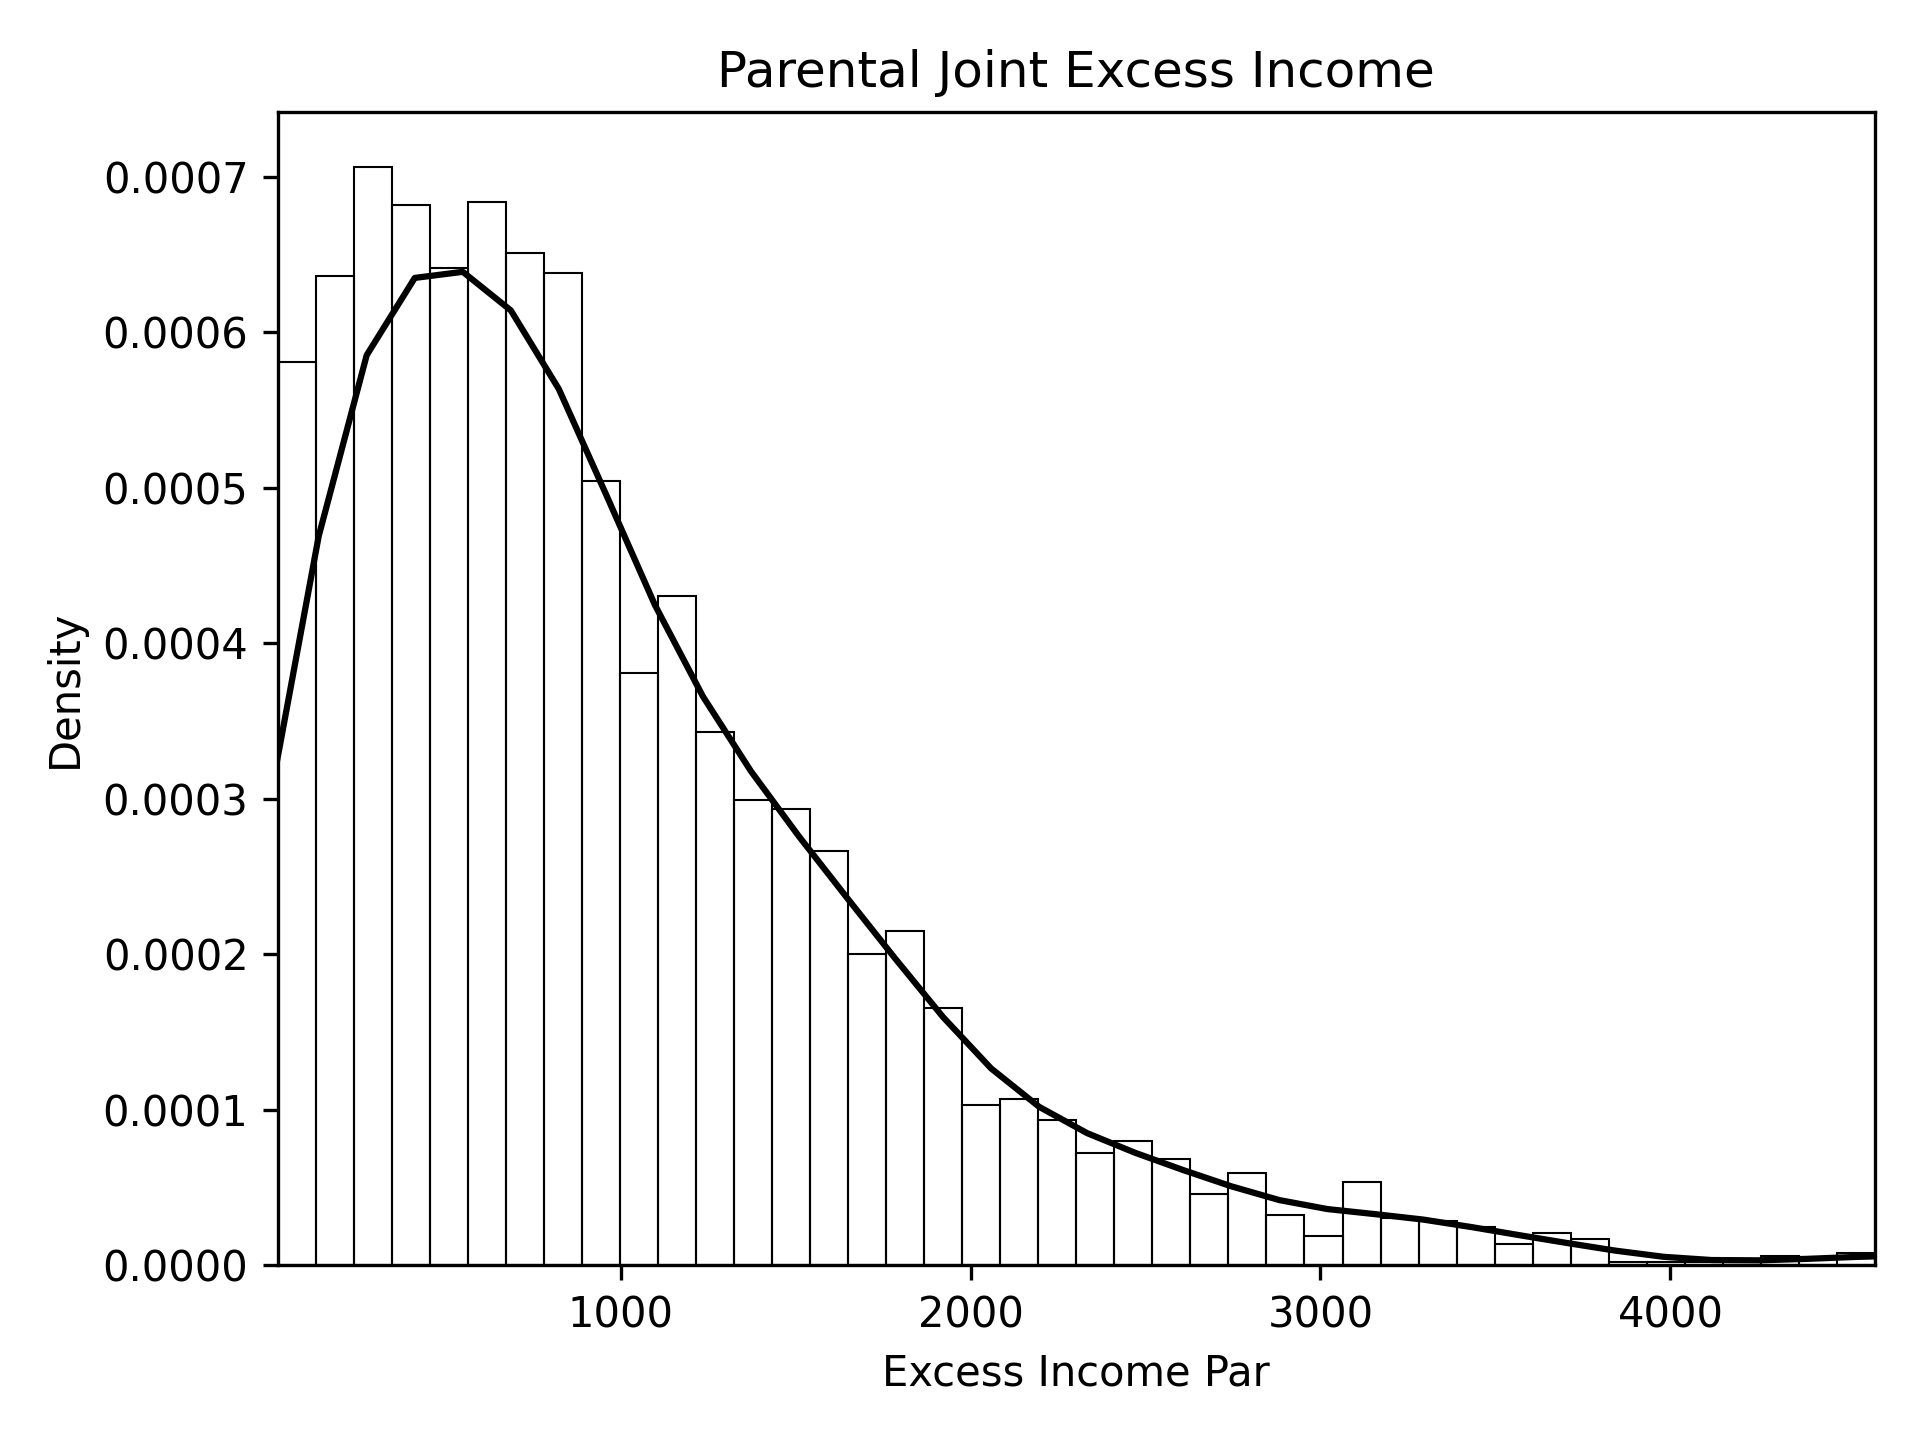
\includegraphics[width=\linewidth]{parental_joint_excess_income_pdf.png}
    \caption{Parental joint excess income}
    \label{fig:parental-excess}
  \end{subfigure}
  \hfill
  \begin{subfigure}[t]{0.48\linewidth}
    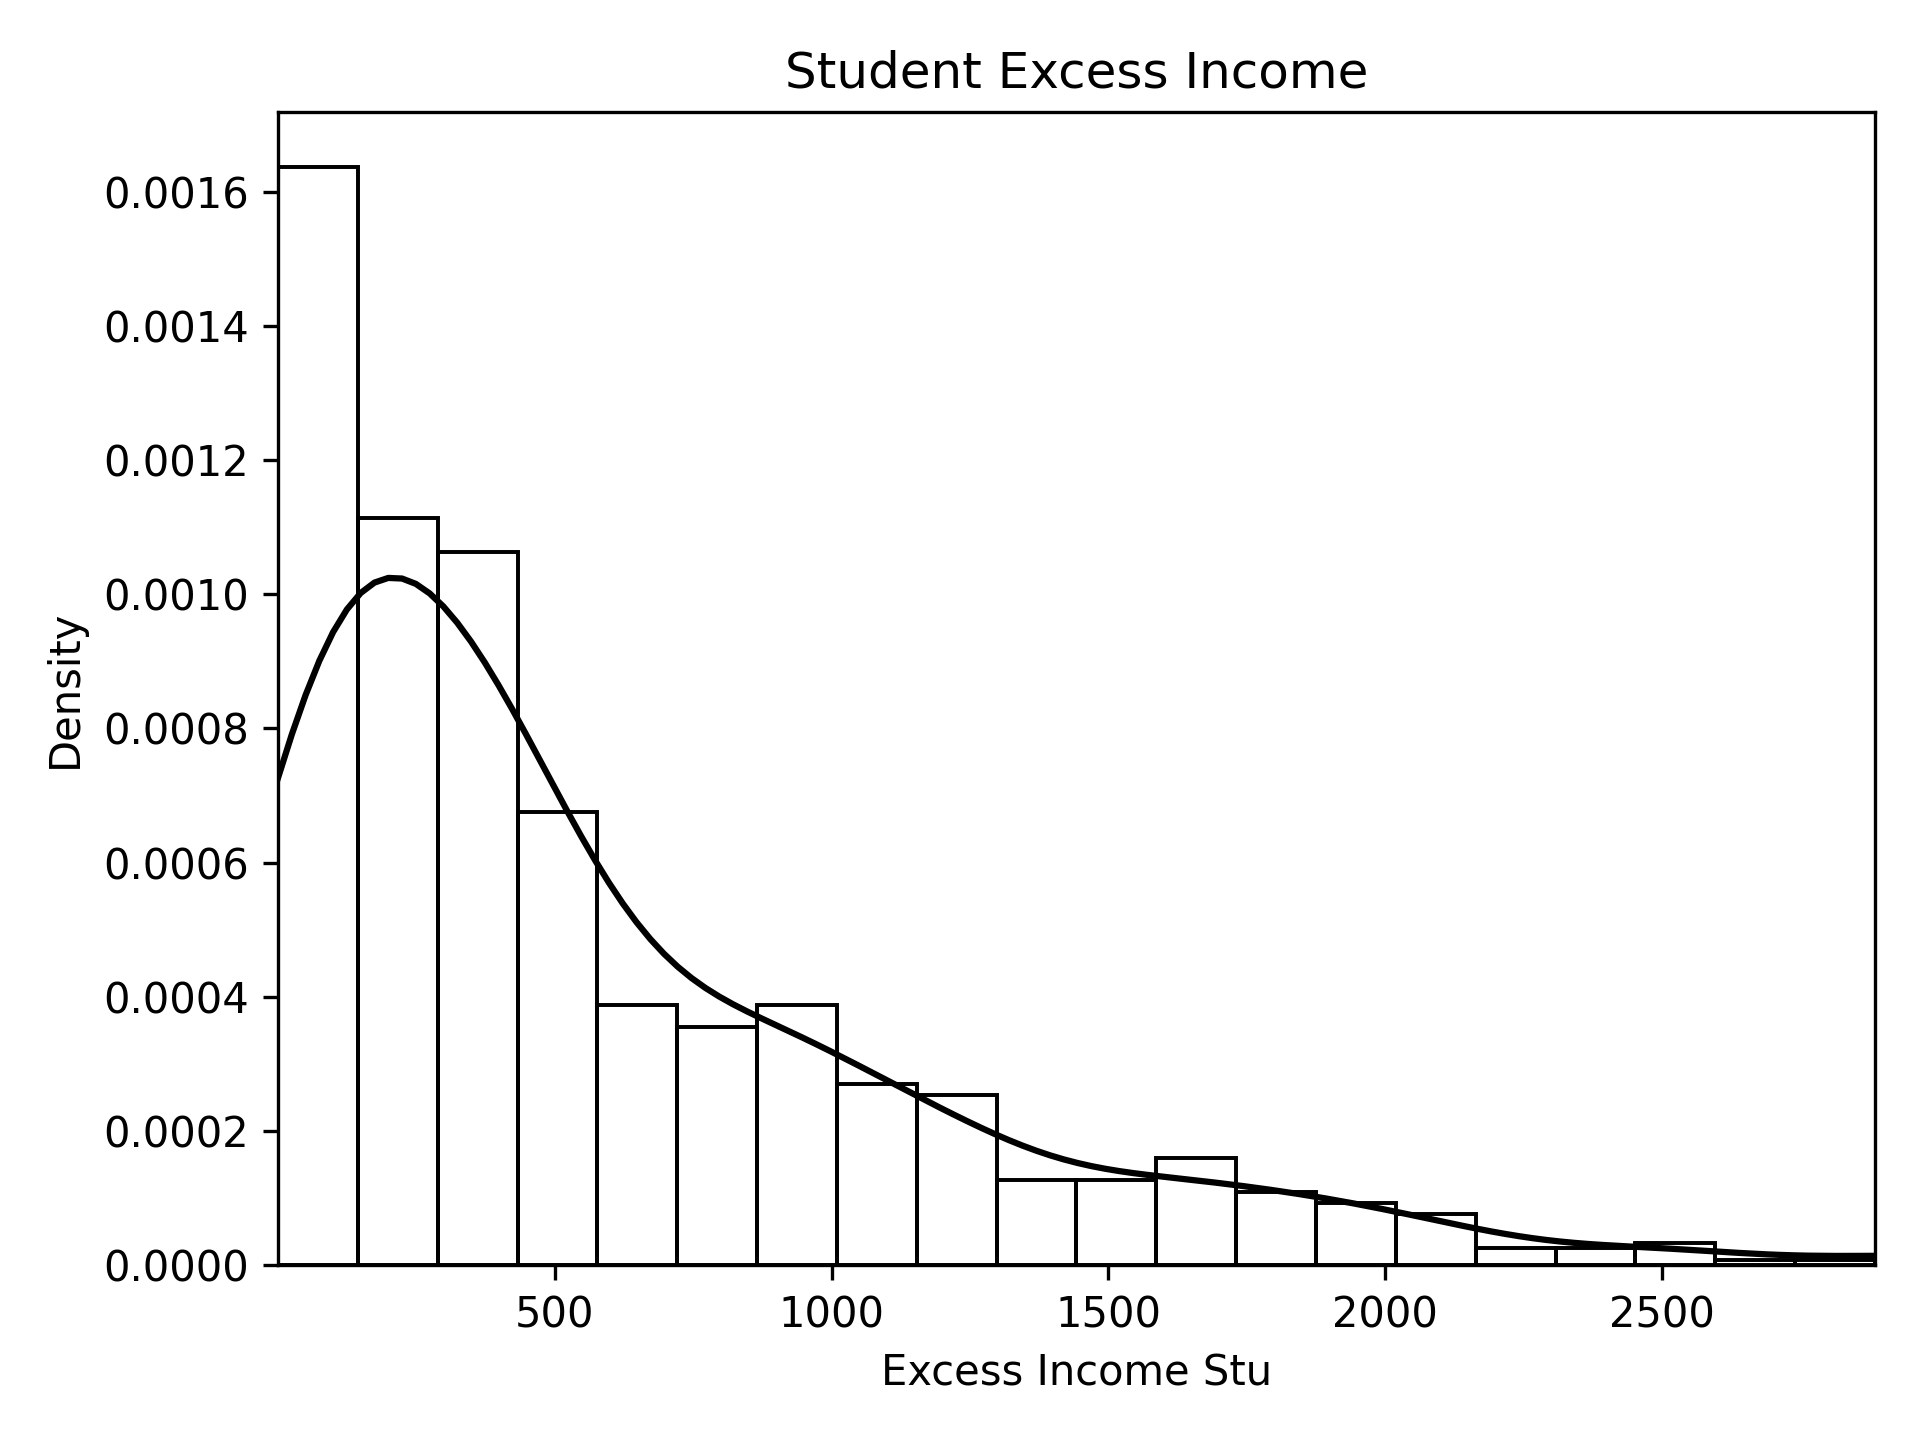
\includegraphics[width=\linewidth]{student_excess_income_pdf.png}
    \caption{Student excess income}
    \label{fig:student-excess}
  \end{subfigure}
  \caption{Simulated mean excess income for parents (\subref{fig:parental-excess}) and students (\subref{fig:student-excess}).}
  \label{fig:excess-income}
\end{figure}

\begin{figure}[htbp]
  \centering
  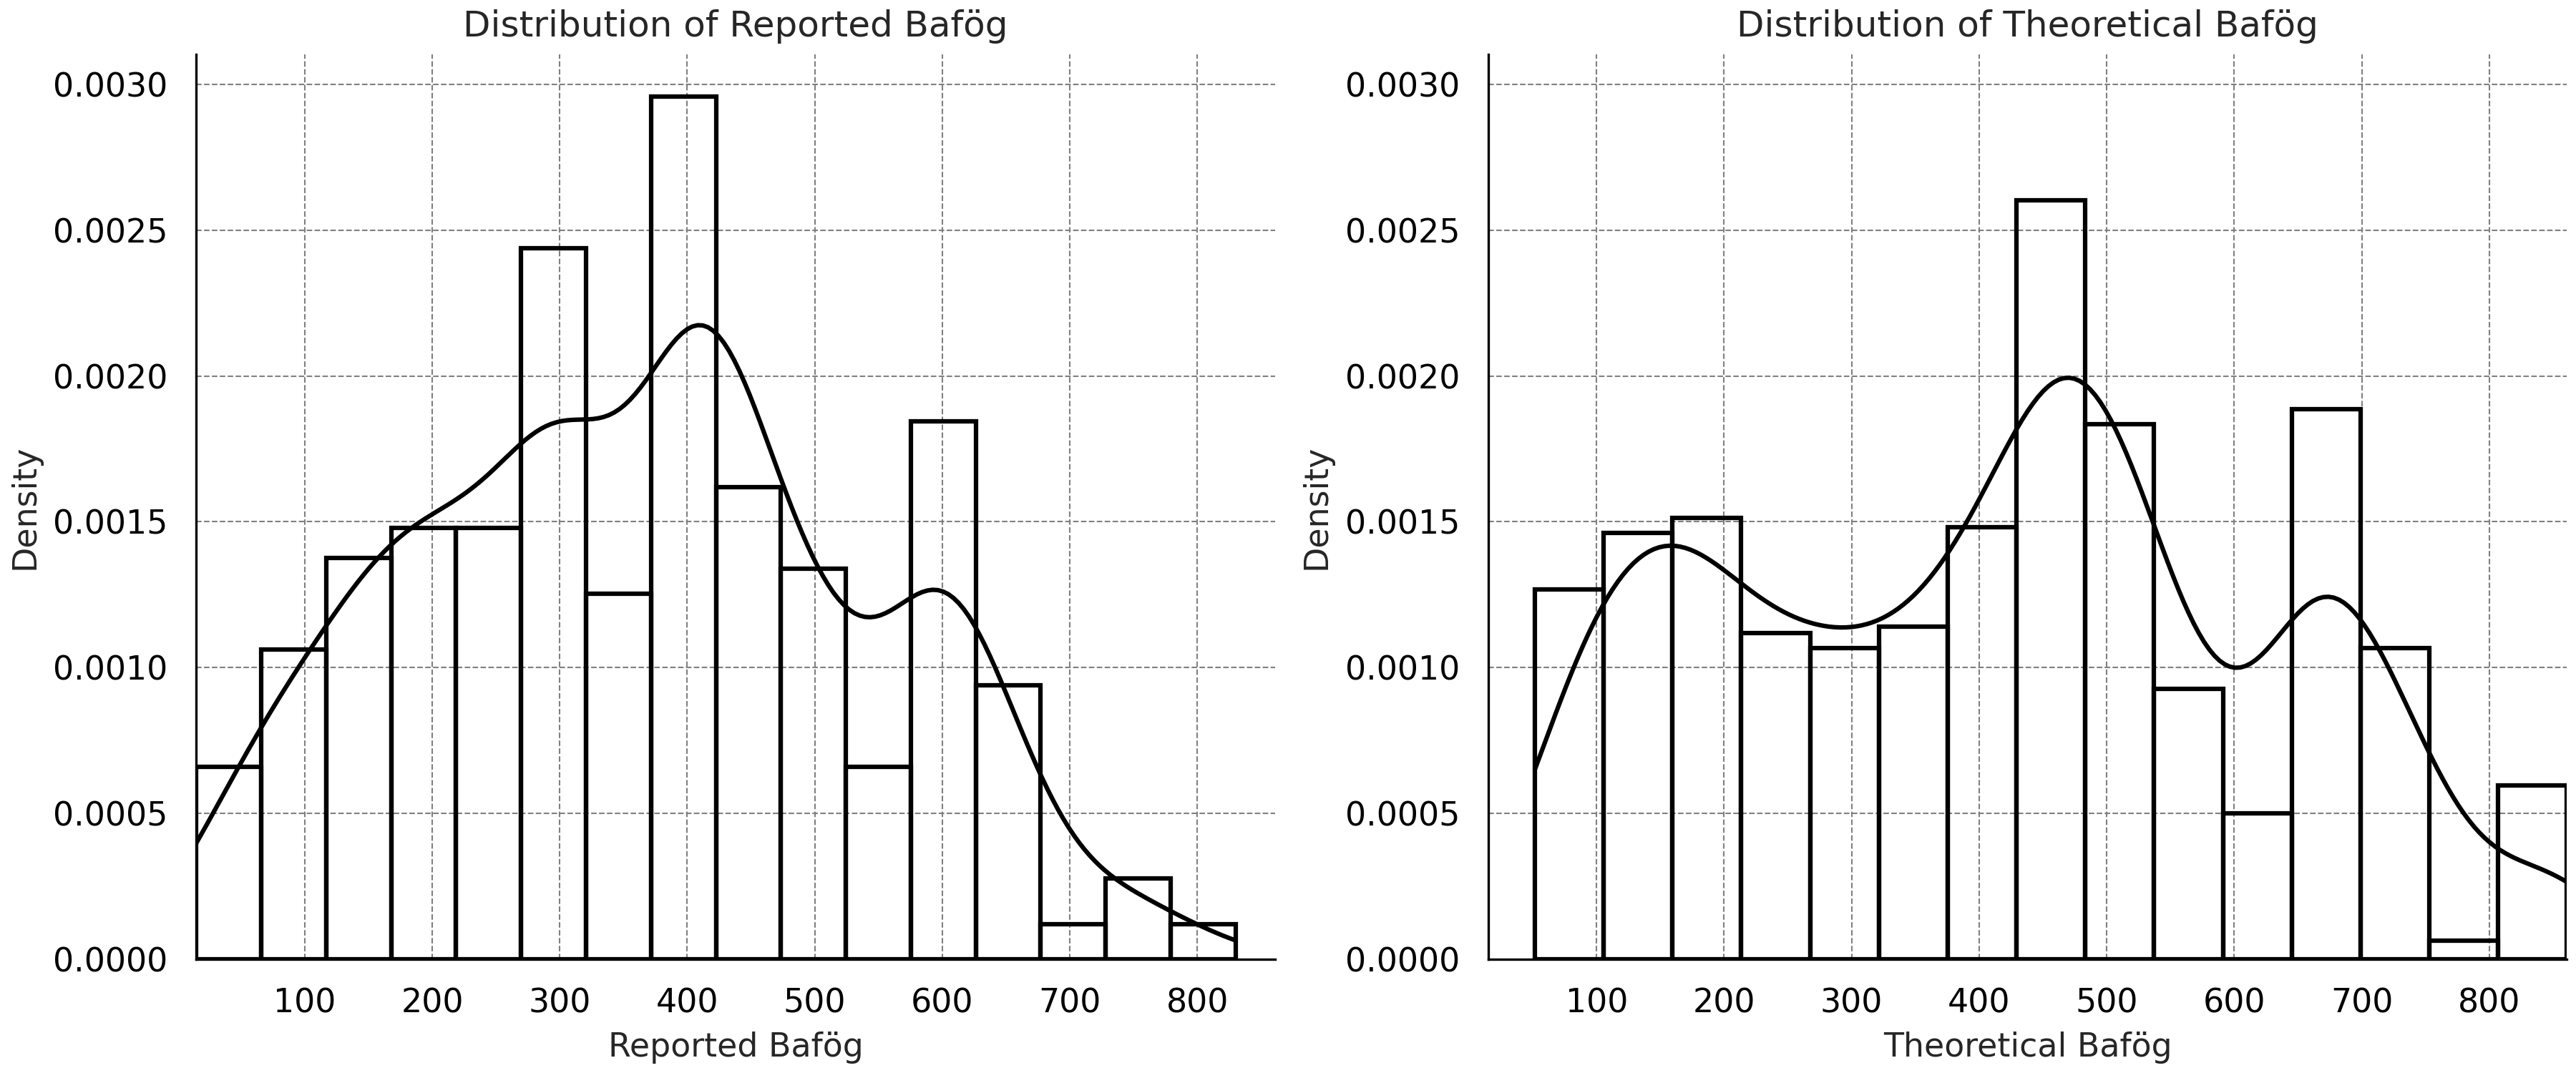
\includegraphics[width=0.95\linewidth]{theo_vs_reported_distribution.png}
  \caption{Comparison of the distribution of reported BAföG receipt in the SOEP-Core sample with the simulated (theoretical) distribution of simulated BAföG entitlements from our model.}
  \label{fig:theo-vs-reported}
\end{figure}

\subsection{Determinants of Non-take-up}
\subsubsection{Binary Choice Model}

\begin{table}[htbp]
\centering
\footnotesize
\caption{Logit and Probit coefficients and AMEs (Average Marginal Effects). Significance: *\( p < 0.1 \), **\( p < 0.05 \), ***\( p < 0.01 \)}
\label{tab:logit-probit-ame}
\begin{tabular}{lllllll}
\toprule
             & \multicolumn{3}{c}{Logit}           & \multicolumn{3}{c}{Probit} \\
\cmidrule(lr){2-4} \cmidrule(lr){5-7}
             & Coef.    & AME      & Std. Err.   & Coef.    & AME      & Std. Err. \\
\midrule
Intercept                           & -1.702    &            & 1.14     & -1.070    &            & 0.67     \\
Age                                 & 0.133***  & 0.028***   & 0.03     & 0.080***  & 0.028***   & 0.02     \\
Sibling BAföG                       & -0.460*** & -0.096***  & 0.16     & -0.279*** & -0.096***  & 0.10     \\
East                                & -1.233*** & -0.258***  & 0.20     & -0.752*** & -0.259***  & 0.12     \\
gmi 100                             & 0.061**   & 0.013**    & 0.03     & 0.035**   & 0.012**    & 0.01     \\
has partner                         & 0.104     & 0.022      & 0.53     & 0.065     & 0.023      & 0.31     \\
Parents (Lower Secondary Education) & 0.340     & 0.071      & 0.62     & 0.236     & 0.081      & 0.38     \\
isced3                              & 0.396     & 0.083      & 0.58     & 0.263     & 0.091      & 0.35     \\
isced4                              & 0.426     & 0.089      & 0.59     & 0.285     & 0.098      & 0.36     \\
isced5                              & 0.720     & 0.151      & 0.64     & 0.474     & 0.163      & 0.39     \\
isced6                              & 0.644     & 0.135      & 0.60     & 0.425     & 0.146      & 0.37     \\
isced7                              & 2.249***  & 0.470***   & 0.79     & 1.388***  & 0.478***   & 0.47     \\
isced8                              & 1.493     & 0.312      & 1.27     & 0.946     & 0.326      & 0.79     \\
lives at home                       & 0.293     & 0.061      & 0.20     & 0.186     & 0.064      & 0.12     \\
Direct migration background         & -0.186    & -0.039     & 0.26     & -0.108    & -0.037     & 0.16     \\
Indirect migration Background       & -0.380*   & -0.079*    & 0.20     & -0.231*   & -0.080*    & 0.12     \\
Parental Income                     & -0.029**  & -0.006**   & 0.01     & -0.018**  & -0.006**   & 0.01     \\
Risk Apetite                        & 0.018     & 0.004      & 0.02     & 0.011     & 0.004      & 0.01     \\
Sex                                 & -0.091    & -0.019     & 0.16     & -0.048    & -0.017     & 0.10     \\
Simulated BAföG                     & -0.112*   & -0.023*    & 0.06     & -0.067*   & -0.023**   & 0.03     \\
\bottomrule
\end{tabular}
\end{table}


\paragraph{Risk attitudes.} In this analysis, a variable for students' self-assessed willingness to take risks is included. Even though BAföG offers relatively safe and generous conditions, some students might still be hesitant to take on any form of debt if they are generally risk-averse. By including this variable, we aim to capture whether differences in individual risk preferences help explain why some eligible students choose not to apply.

Herber and Kalinowski (2016) also include a risk preference variable in their study, mainly to control for the possibility that risk attitudes could affect take-up behavior or influence how other factors, like impatience, play a role. They do not find a strong effect of risk aversion on BAföG take-up, but they still argue it is useful to control for \citep{herber_non-take-up_2019}. In a similar way, we include this variable to improve our model and to see whether risk aversion plays any role in students’ decisions to reject BAföG.

\paragraph{East German socialization.}  A variable indicating whether the student lives in East Germany is included to account for potential differences in attitudes toward state support rooted in historical and regional context. Alesina and Fuchs-Schündeln (2007) show that individuals from the former GDR tend to have stronger preferences for redistribution and a greater belief in the role of the state in providing social services, and that these differences in preferences can persist for one to two generations after reunification \citep{alesina_good-bye_2007}. Current residence in East Germany may reflect continued exposure to these norms and institutions and can serve as a reasonable proxy for this form of socialization. Since the variable is statistically significant at the 5\% level in our model, we interpret it as capturing persistent regional differences in how students view and respond to publicly provided financial support like BAföG.




